\chapter{Aplikace metod}

V této kapitole se zabýváme aplikováním a porovnáváním metod, kterým jsme se věnovali v kapitole \ref{chap:reseniOptUloh}.
Namodelujeme pohotovostní službu a synteticky vytvoříme sadu incidentů, pro kterou budeme hledat optimální pohotovostní plán.
V rámci této práce namodelujeme pražskou záchranou službu pro rok 2017. Budeme vycházet z veřejně dostupných dat
poskytnutých přímo zdravotnickou záchrannou službou hlavního města Prahy
\footnote{https://www.zzshmp.cz/wp-content/uploads/2017/12/Statistiky-160let-ZZSHMP.pdf}.
Především nás bude zajímat kvalita nalezených optimálních plánů a rychlost jejich nalezení.

\section{Generování dat}

Nejprve vygenerujeme data reprezentující výjezdové stanice a nemocnice, čímž namodelujeme pohotovostní službu.
Ty můžeme vygenerovat libovolně, ale z důvodu praktičtějšího využití
si v této prácí vybereme jako pohotovostní službu pražskou záchrannou službu.
Pražská záchranná služba disponuje 20 výjezdovými stanicemi a 140 vozidly.
Údaje o počtu záchranných týmu nejsou veřejně dostupné. Jedinou dostupnou informací je celkový počet zaměstanců, který činí přes 500 lidí.
Tam ale spadají i nezáchranáři.
V Praze se nachází 12 nemocnic.

Nyní namodelujeme incidenty. Podle statistik zveřejněných pražskou záchrannou službou se v roce 2017 v Praze denně uskutečnilo průměrně na 330 výjezdů.
Nejrušnější část všedního dne je mezi 9 a 12 hodinou, kdy se odehrává až dvojnásobně incidentů než je průměr.
Incidenty se odehrávají mnohem častěji ve středu Prahy, než v jejím okolí. 

Podle těchto informací namodelujeme sadu incidentů.
V první řadě si území Prahy reprezentujeme jako mnohoúhleník a pomocí normálního rozdělení vygenerujeme souřadnice v něm obsažené.
Normálnímu rozdělení nastavíme střední hodnotu na střed mnohoúhelníka a směrodatnou odchylku nastavíme tak, aby se incidenty na okrajích Prahy odehrávaly méně než v centru. 
Kde a v kolik hodin se incidenty odehrávají přesně záchranná služba Prahy nezveřejňuje, pravděpodobně proto, že by se mohlo jednat o zneužitelné nebo citlivé údaje.
Rozloha Prahy činí 496 kilometrů čtverečních a je relativně symetrického tvaru. Pro naše účely tak bude stačit nastavit směrodatnou odchylku na 10 kilometrů.
Incidenty jsou vygenerovány tak, aby se děly častěji mezi 9 a 12 hodinou, a odpovídaly tak skutečnosti.

\begin{figure}[H]
  \caption{Záchranná pohotovostní služba a nemocnice spolu s incidenty na mapě Prahy.}
  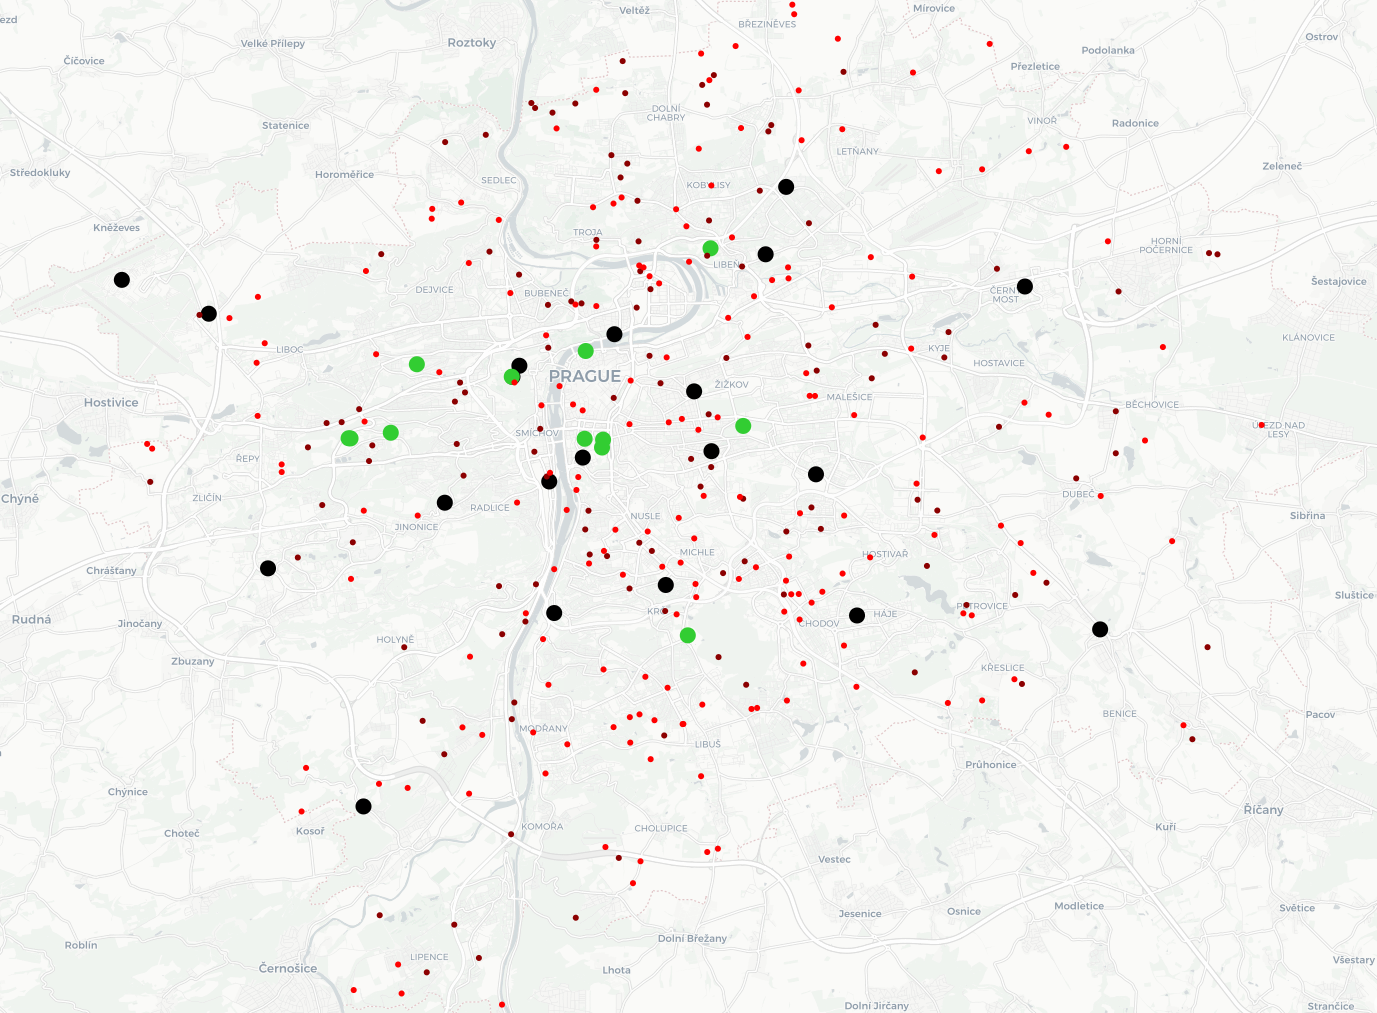
\includegraphics[width=\textwidth]{img/prague_monday_420.png}
  \centering
  \label{img:prague}
\end{figure}

Na obrázku \ref{img:prague} je znázorněna mapa Prahy s rozmístěnými 20 výjezdovými stanicemi (body černé barvy), 12 nemocnicemi (body zelené barvy) a 300 incidenty (body červené barvy).
Tmavě červené body reprezentují incidenty, které se odehrají mezi 9 a 12 hodinou.

S výše popsanou reprezentací pohotovostní služby a sadou incidentů je třeba zajistit, aby simulace uměla věrohodně zjistit dobu trvání každého příjezdu.
Připomeňme si, že simulaci používáme právě z toho důvodu, aby počet úspěšně odbavených incidentů plánem byl co nejvěrohodnější.
Věrohodnost zajistíme použitím Google APIs, která nám pomohou zjistit doby všech příjezdů. Konkrétně použitím Distance Matrix API a Routes API.

V průběhu simulace je potřeba především znát následující doby příjezdů:
\begin{enumerate}
  \item z výjezdové stanice na incident,
  \item z incidentu do nemocnice,
  \item z nemocnice zpět na výjezdovou stanici.
\end{enumerate}

Simulace podporuje i tzv. \textit{reroute}, tedy v momentě, kdy se záchranný tým vrací po odbavení incidentu zpět na výjezdovou stanici,
tak je povoleno, aby mohl z aktuální lokace vyrazit na odbavování dalšího incidentu, aniž by se musel vracet zpět na výjezdovou stanici.

Doby příjezdů mezi výjezdovými stanicemi, incidenty a nemocnicemi si můžeme předpočítat, ale \textit{reroute} předpočítat nelze.
Můžeme si alespoň v průběhu simulování všechny spočítané doby příjezdů mezi lokacemi udržovat s přesností na desítky metrů,
aby se v budoucnu nemuselo volat Google API. To je samozřejmě pomalá operace, trvající desítky až stovky milisekund. 

\section{Aplikace naivního řešení}

První metodu, kterou aplikujeme na namodelovanou záchrannou službu a incidenty dle předchozí kapitoly je naivní řešení.

\begin{figure}[H]
  \caption{Nalezené plány naivním řešením.}
  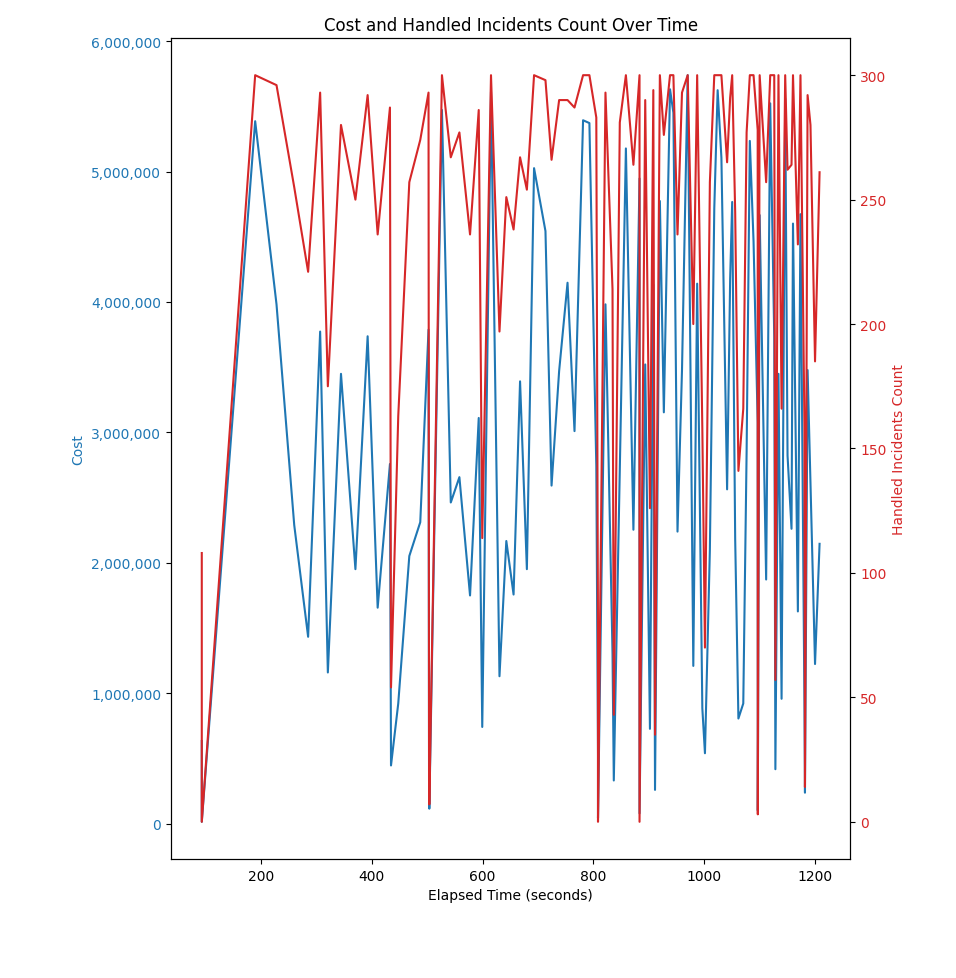
\includegraphics[width=\textwidth]{img/plots/naive.png}
  \centering
  \label{img:naive}
\end{figure}

Na grafu \ref{img:naive} vidíme naivní řešení spuštěné po dobu 20 minut.
Naivní řešení pouze náhodně generuje pohotovostní plány a vyhodnocuje je při účelové funkci. Můžeme vidět, že nalezené plány velmi kolísají jak v ceně tak v počtu odbavených incidentů. 
Naivní řešení není nijak více zajímavé a nebudeme jej dále zkoumat. Slouží spíše jako základ, se kterými můžeme porovnávat lepší metody, diskutované níže. 

\section{Aplikace prohledávání plánů optimálními tahy} \label{kap:aplikaceTabu}

V této kapitole aplikujeme algoritmus prohledávání plánů optimálními tahy \ref{alg:rekProhPlanu}.
Konkrétně použijeme jeho mírně upravenou verzi, diskutovanou na závěru kapitoly \ref{kap:rekurzivniProhledavaniStromu},
kde strom tahů budeme prohledávat vždy od prázdného plánu, a na každé hladině rekurze zvolíme pouze jeden náhodný optimální tah.

\begin{table}[h!]
\centering
\begin{tabular}{|c|c|c|}
\hline
\textbf{Čas běhu v minutách} & \textbf{Cena plánu} & \textbf{Odbavené incidenty} \\
\hline
7:11 & 2455260 & 292 \\
\hline
  \textbf{10:53} & \textbf{2469661} & \textbf{296} \\
\hline
13:38 & 2433659 & 294 \\
\hline
16:28 & 2347256 & 294 \\
\hline
19:23 & 2376058 & 293 \\
\hline
22:06 & 2340053 & 290 \\
\hline
25:14 & 2433661 & 292 \\
\hline
28:13 & 2368858 & 293 \\
\hline
30:46 & 2404856 & 294 \\
\hline
33:08 & 2448061 & 291 \\
\hline
\end{tabular}
\caption{Spuštění prohledávání optimálními tahy na modelu Prahy.}
\label{table:optimalMovesTabulka}
\end{table}

Po spuštění metody na modelu Prahy po dobu kolem 30 minut metoda navštívila 10 plánů dosažitelných optimálními tahy.
Celkově při budování těchto 10 plánů však navštívila něco přes $300 \cdot 10 = 3000$ plánů, protože algoritmus plány buduje postupně podle incidentů (viz algoritmus \ref{alg:rekProhPlanu}).
Nalezený optimální plán odbavuje 296 incidentů a stojí 2469661 (viz tabulka \ref{table:optimalMovesTabulka}).
Dále má naalokovaných 100 týmů a 61 záchranných vozidel.

První plán trvá nalézt nejdéle, něco přes 7 minut. Důvodem je, že \textit{cache} dob příjezdů obsahuje pouze předpočítané hodnoty a musí se vykonávat větší množství
dotazů na Google API.
Při prohledávání dalších plánů už se dotazuje na Google API mnohem méně často.
Pro zajímavost, celkový počet dotazů na dobu trvání příjezdu je 133189050, kde pro 133179688 případu, tedy $99.99\%$, byla doba příjezdu předpočítaná a vrácena z \textit{cache}.
Podobně se \textit{cache} chová i u ostatních metod.

\section{Aplikace lokálního prohledávání}

V této kapitole aplikujeme na model Prahy lokální prohledávání (viz kapitola \ref{kap:localSearch}).
Metodu použijeme přesně jak je popsaná algoritmem \ref{alg:hillclimb}.
Prohledávání začneme z prázdného plánu a jako účelovou funkci použijeme váženou sumu ceny plánu a počtu odbavených incidentů, s parametrem $\alpha = 0.99$ (viz definice \ref{df:vazenaSumaUcelF}),
abychom upřednostňovali plány s vyšším počtem odbavených incidentů.
Jakou přesně účelovou funkci si zvolíme uvážíme podle toho, co pro nás konkrétně znamená optimální plán.
My budeme chtít zkoumat především plány odbavující co nejvíce incidentů, a až poté minimalizovat cenu.

Potřebujeme ještě nadefinovat jak budou vypadat sousedi nějakého plánu.
Ty standardně nadefinujeme implicitně pomocí tahů a vyžadujeme, aby splňovali alespoň nutné podmínky.
Takové tahy můžeme vybrat různě, my si vybereme tahy uvedené jako příklad tahů, které nutné podmínky splňují (viz příklad \ref{pr:sousedi}).

Záměrně alokování týmu a vozidla zvolíme jako jeden tah a nikoliv jako dva samostatné tahy. Vyhneme se tak situaci, kdy by se lokální prohledávání zastavilo v lokálním optimu, 
kde už nelze odbavit žádný incident naalokování týmu a vozidla odděleně, ale pouze zároveň.
Takové lokální optimum by pak bylo suboptimální, protože by odbavovalo méně incidentů, než by mohlo být možné.
Takto definované sousedství budeme používat i u dalších metod.

\begin{figure}[H]
  \caption{Nalezené plány metodou lokálního prohledávání plánů.}
  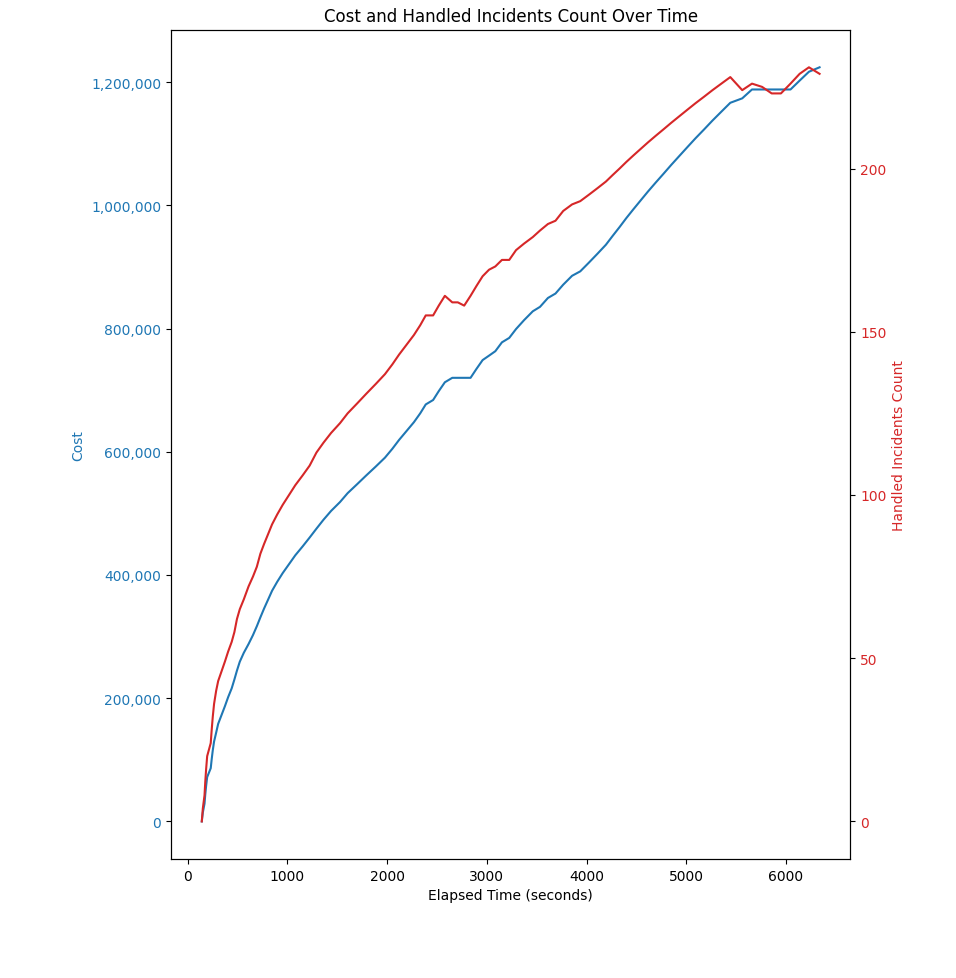
\includegraphics[width=0.7\textwidth,height=0.7\textwidth]{img/plots/localSearch_empty.png}
  \centering
  \label{img:localSearchRes}
\end{figure}

Na grafu \ref{img:localSearchRes} vidíme jak se aktuální plán mění v čase.
Lokální prohledávání bylo spuštěné po dobu 50 minut, a pak bylo přeřušeno. 
Nejlepší nalezený plán po hodině a půl úspěšně odbaví 229 incidentů z 300 incidentů a stojí 1224080.
Lokální prohledávání celkem navštívilo 29248 plánů. To je až 7 krát tolik, kolik plánů navštívila metoda prohledávání optimálními tahy.

I když se podle růstu křivky dá usoudit, že by metoda lokálního prohledávání byla schopná nalézt dost dobrý plán, trvalo by to příliš dlouho.
Můžeme si polepšit, sice tak, že začneme prohledávát ne z prázdného plánu, ale z plánu zvoleného nějak chytře.
Z plánu, který už je skoro optimální a lokální prohledávání už jej jenom doladí.

Jednou z možností jak takový startovní plán zvolit je použít první nalezený optimální plán předchozí metodou, a na něj spustit lokální prohledávání.

\begin{figure}[H]
  \caption{Nalezené plány metodou lokálního prohledávání plánů z plánu nalezeného optimálními tahy.}
  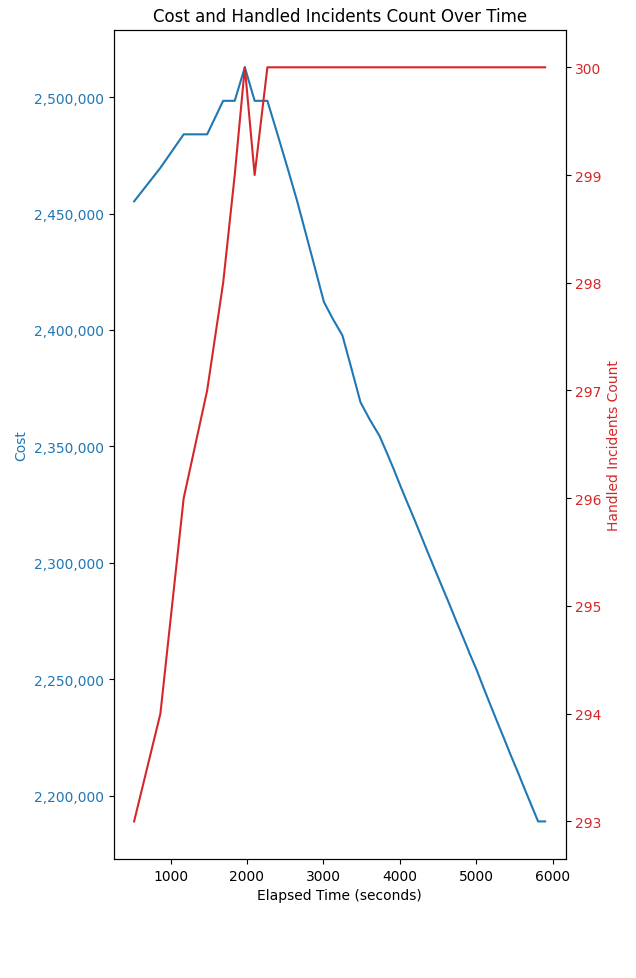
\includegraphics[width=0.7\textwidth,height=0.9\textwidth]{img/plots/localSearch_fromOptimal.png}
  \centering
  \label{img:hybrid}
\end{figure}

Na grafu \ref{img:hybrid} vidíme lokální prohledávání začínající ne z prázdného plánu, ale z plánu nalezeného optimálními tahy.
Můžeme vidět, že lokální prohledávání upravuje plán tak, že postupně odbavuje více incidentů, až nakonec všech 300. Poté už jen postupně snižuje cenu plánu.
Po zhruba 30 minutách nalezne plán odbavující všechny incidenty a do hodiny a půl lokální prohledávání stagnuje a nalezne lokální optimum.
Optimální nalezený plán odbavuje všech 300 incidentů, stojí 2188863 a má naalokovaných pouze 88 týmů a 63 vozidel.

\section{Aplikace tabu prohledávání}

V této kapitole aplikujeme na model Prahy tabu prohledávání (viz kapitola \ref{kap:tabuSearch}).
Tabu prohledávání je v podstatě lokální prohledávání s pamětí, podle které umí sofistikovaněji vybrat sousední plán,
pokud se ocitne v lokálním optimu.

\begin{figure}[H]
  \caption{Nalezené plány tabu metodou z prázdného plánu.}
  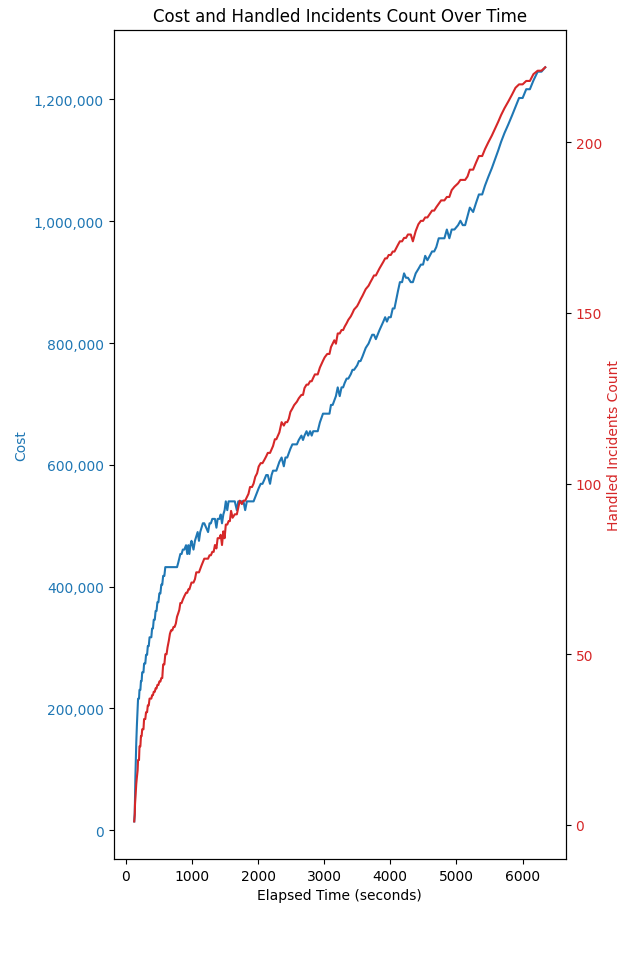
\includegraphics[width=0.7\textwidth,height=0.9\textwidth]{img/plots/tabuSearch_empty.png}
  \centering
  \label{img:empty_tabu}
\end{figure}

Z toho důvodu bude podobně jako u lokálního prohledávání (viz graf \ref{img:empty_tabu}) trvat příliš dlouho, než nalezne nějaký dost dobrý plán.

\begin{figure}[H]
  \caption{Nalezené plány tabu metodou z plánu nalezeného optimálními tahy.}
  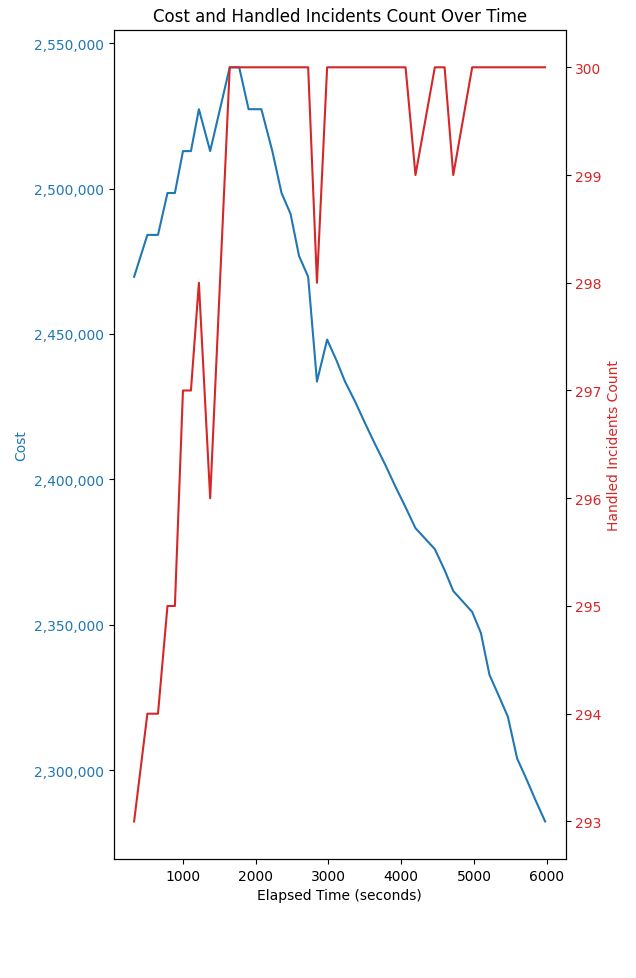
\includegraphics[width=0.7\textwidth,height=0.9\textwidth]{img/plots/tabuSearch_fromOptimal.png}
  \centering
  \label{img:hybrid_tabu}
\end{figure}

Na grafu \ref{img:hybrid_tabu} vidíme doposud nejlepší plány nalezené tabu metodou v čase z plánu nalezeného optimálními tahy. 
Nalézt plán odbavující všech 300 incidentů trvá kolem 40 minut, což je o 10 minut déle, než trvalo lokálnímu prohledávání. 
To je pochopitelné, protože při navštívení každého souseda, kterých bude obdobně jako u lokálního prohledávání, se musí kontrolovat,
zda není obsažen v tabu. Proto vyhodnocení souseda bude trvat o něco déle, což se při tak velkém množství navštívených plánů poměrně rychle nasčítá.

Tabu prohledávání bylo puštěno něco kolem hodiny a půl, a obdobně jako u lokálního prohledávání, s roustoucí délkou běhu programu se i snižuje cena plánu.
Výhoda tabu prohledávání je hlavně v schopnosti nezůstat v lokálním optimu a umět robustněji prohledávat prostor konfigurací.
Tato výhoda v našem případě ale není využita, protože tabu prohledávání ani za hodinu běhu na lokální optimum nenarazilo.
Spíše naopak, prohledávání tabu je nevýhodou, protože zbytečně kontroluje tabu, a lokální prohledávání je v tomto případě lepší volbou.

\section{Aplikace simulovaného žíhání}

V této kapitole aplikujeme na model Prahy simulované žíhání (viz kapitola \ref{kap:tabuSearch}).
Simulovanému žíhání je potřeba nastavit následující hyperparametry:
\begin{enumerate}
  \item počáteční teplota,
  \item koncová teplota,
  \item chladící rozvrh,
  \item počet iterací v rámci stejné teploty.
\end{enumerate}

Počáteční teplotu je vhodné nastavit tak, aby pravděpodobnost přijetí horší konfigurace byla ze začátku kolem 0.8--0.9 procent \cite{sa_theory}.
Vzhledem k tomu, že používáme váženou sumu účelových funkcí, tak se výsledná hodnota účelové funkce pohybuje mezi 0 a 1.
Tím pádem rozdíl se pohybuje mezi -1 a 1.
Pokud je $\Delta$ záporná, tak je sousední plán vždy navštíven, protože je
jeho hodnota při účelové funkci vyšší. Zajímá nás tedy pouze případ, kdy je $\Delta$ nekladná.

Připomeňme si jak vypadá akceptační kritérium:
\begin{align*}\label{df:metropolis}
  \exp\left(-\frac{\Delta q}{t}\right).
\end{align*}

Počáteční teplota splňující takový požadavek činí například 5 stupňů, jak můžeme vidět na obrázku \ref{img:metropolis_5},
kde na ose x je hodnota delta, a na ose y pravděpodobnost přijetí sousedního plánu metropolisním kritériem, který se od aktuálního liší o danou deltu.

\begin{figure}[H]
  \centering
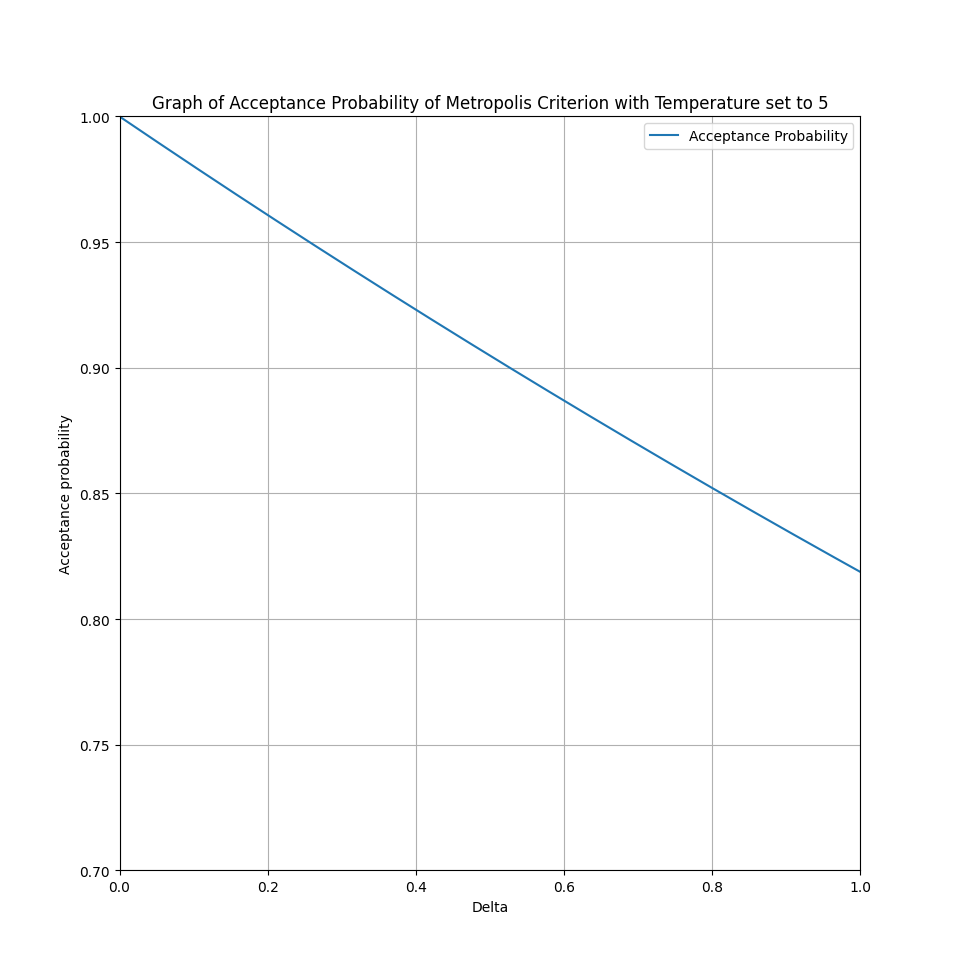
\includegraphics[width=0.5\textwidth,height=0.5\textwidth]{img/metropolis_5.png}
  \caption{Metropolis kritérium pro teplotu 5 stupňů.}
  \label{img:metropolis_5}
\end{figure}

Finální teplota se často volí velmi blízko nule, aby bylo možné dostatečně důkladně prohledat konfigurace lokálně, podobně jak dělá například lokální prohledávání \cite{sa_theory}.
Zatím vyberme finální teplotu jako $10^{-6}$.

Vybrat ochlazovací rozvrh lze různě, nejčastěji používané jsou \cite{sa_theory}:
\begin{enumerate}
  \item Lineární ochlazovací rozvrh, kde se teplota aktualizuje následovně:
    \begin{align*}
      t_{k+1} = t_k - k \cdot \Delta t_k,
    \end{align*}
    kde $t_k$ je aktuální teplota, $t_{k+1}$ je nová teplota a $\Delta t_k$ je hyperpametr, o kolik teplotu snižovat.
    Je velmi jednoduchý na implementaci, ale není tak dobrý jako ostatní ochlazovací rozvrhy \cite{sa_schedules}.

  \item Logaritmický ochlazovací rozvrh:
    \begin{align*}
      t_{k+1} = t_{k} / \log(1 + k).
    \end{align*}
    Logaritmický ochlazovací rozvrh má dobré teoretické vlastnosti, ovšem pro praktické použití je příliš pomalý \cite{sa_schedules}.

  \item Exponenciální ochlazovací rozvrh:
    \begin{align*}
      t_{k+1} = t_k \cdot \alpha,
    \end{align*}
    kde $\alpha$ se často volí mezi 0.8 a 0.99 \cite{sa_theory}.
    Podobně jako předchozí ochlazovací rozvrhy je velmi jednoduchý na implementaci, a často bývá dobrou první volbou, protože umí najít dobrý balanc mezi explorační fází,
    kdy je teplota vyšší a mezi ladící fází, kdy je teplota nižší \cite{sa_theory}.

  \item Adaptující se ochlazovací rozvrh. Algoritmus si sám v průběhu nastavuje teplotu podle doposud nalezených konfigurací.
    Náročnější na implementaci než předchozí ochlazující rozvrhy. Hodí se uvažovat o jeho použití především, pokud jednodušší ochlazující rozvrhy nalézají pouze suboptimální řešení.
\end{enumerate}

My si jako ochlazovací rozvrh zvolíme exponenciální ochlazovací rozvrh, především pro jeho jedhoduchou implementaci a pěkné vlastnosti.
Parametr $\alpha$ určující rychlost snižování teploty zatím zvolíme jako $0.99$.

Nelze obecně říct, kolik iterací $M_k$ provést v rámci stejné teploty. Menší počet iterací může vést k předčasné kovergenci, ale na druhou stranu je výpočet méně náročný. \cite{sa_theory}. 
Zvolme zatím pouze jednu iteraci, čili $M_k = 1$.
Samozřejmě, že ideální je použít $\alpha$ rovno $0.99$ a $M_k$ velmi vysoké, například v rámci stovek až tisíců, 
ovšem simulované žíhání s takto zvolenými parametry je velmi výpočetně náročné a běh by trval příliš dlouho.
Z toho důvodu je vhodné balancovat $M_k$ s $\alpha$, pro zajištění rozumné výpočetní náročnosti.

Jako první spustíme simulované žíhání z prázdného plánu.

\begin{figure}[H]
  \caption{Simulované žíhání z prázdného plánu.}
  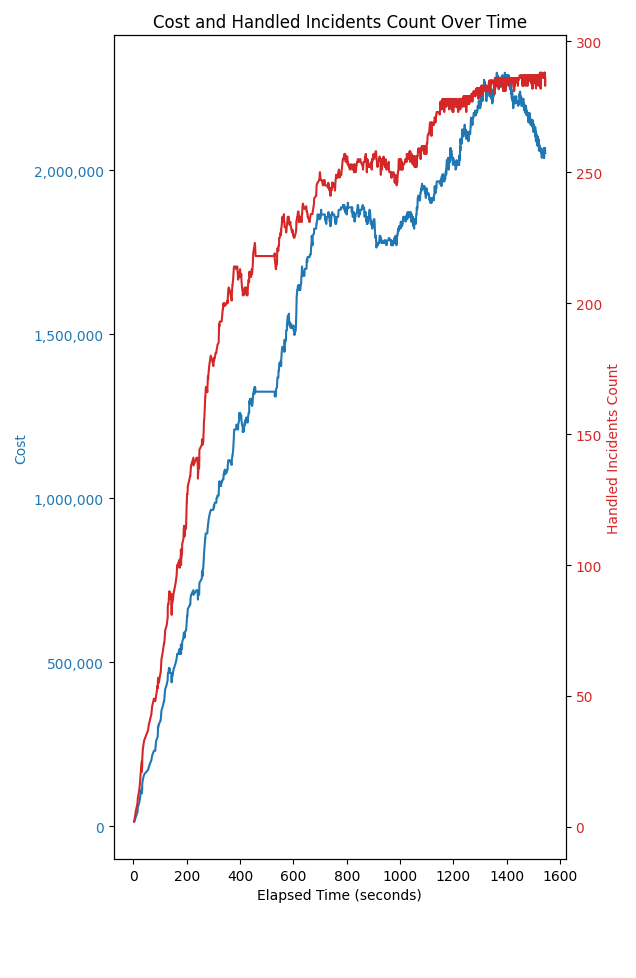
\includegraphics[width=0.7\textwidth,height=0.9\textwidth]{img/plots/sa_empty.png}
  \centering
  \label{img:sa_empty}
\end{figure}

Na grafu \ref{img:sa_empty} vidíme, jaké plány simulované žíhání
s počáteční teplotou 5 stupňů, finální teplotou $10^{-6}$, exponenciálním ochlazovacím rozvrhem s $\alpha = 0.99$ a s $M_k = 1$,
v průběhu z prázdného plánu navštěvovalo.
Celkově běželo simulované žíhání 25 minut a navštívilo celkem 1779 plánů.
Nejlepší nalezený plán odbavuje 288 incidentů, stojí 2059332 a má naalokovaných 93 týmů a 132 záchranných vozidel.
V porovnání s lokálním nebo tabu prohledáváním z prázdného plánu se jedná o dramaticky lepší výsledek.

Podobně jako u předchozích metod můžeme zkusit spustit simulované žíhání z jiného než z prázdného plánu.
Zkusme prvně spustit z uniformě náhodně vygenerovaného plánu, který má naalokovaných zhruba 50\% týmů a vozidel.

\begin{figure}[H]
  \caption{Simulované žíhání z náhodného plánu.}
  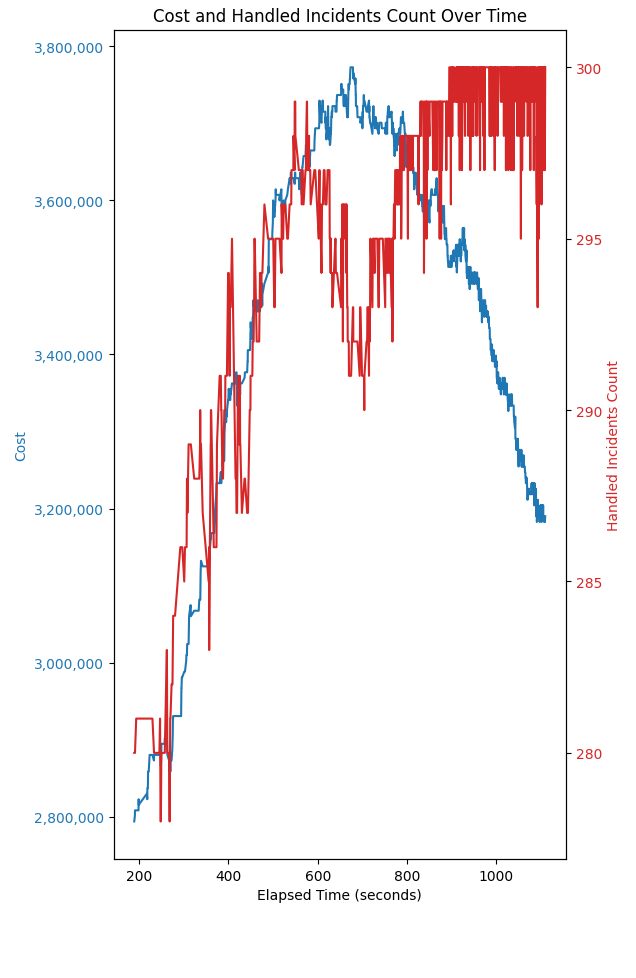
\includegraphics[width=0.7\textwidth,height=0.9\textwidth]{img/plots/sa_random_85.png}
  \centering
  \label{img:sa_random}
\end{figure}

Na grafu \ref{img:sa_random} vidíme chování simulovaného žíhání
s počáteční teplotou 5 stupňů, finální teplotou $10^{-6}$, exponenciálním ochlazovacím rozvrhem s $\alpha = 0.85$ a s $M_k = 10$.
Přibližně do 12 minuty (800 sekund) lze vidět explorační fázi, kdy následně už je plán pouze lokálně vylepšován. 
Spustit simulované žíhání z náhodného plánu přináší lepší výsledky než z plánu prázdného.
Nejlepší nalezený plán odbavuje všech 300 incidentů, stojí 3182531 a má naalokovaných 139 týmů a 126 vozidel.

Z grafu podle klesající ceny můžeme usoudit, že by simulované žíhání bylo schopné najít ještě lepší plán, pokud by mohlo běžet déle.
Spusťmě proto simulované žíhání znovu ze stejného náhodného plánu, tentorkát ale s jinými parametry.

\begin{figure}[H]
  \caption{Simulované žíhání z náhodného plánu.}
  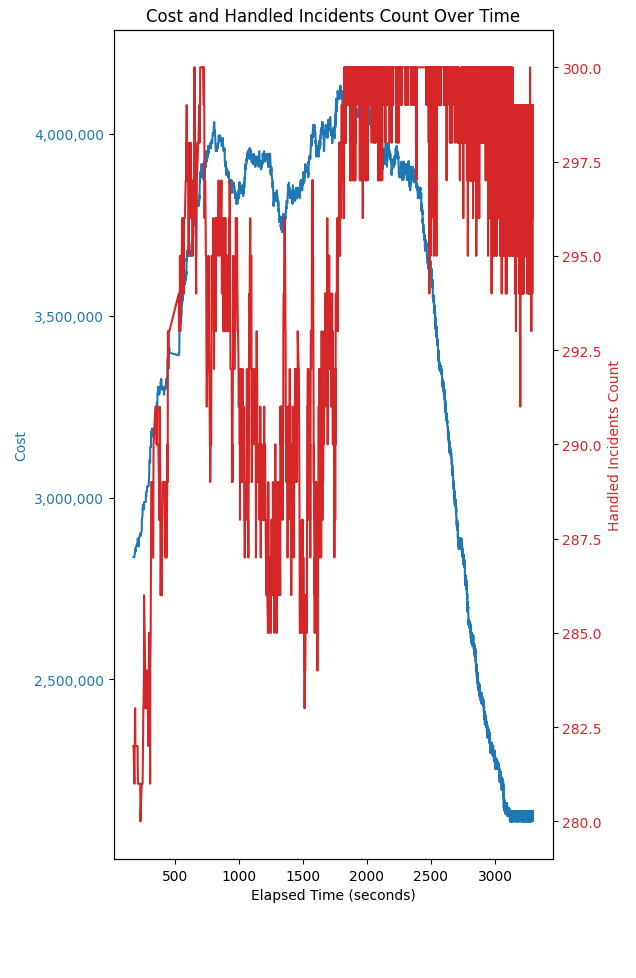
\includegraphics[width=0.7\textwidth,height=0.9\textwidth]{img/plots/sa_random_90.png}
  \centering
  \label{img:sa_random}
\end{figure}

Na grafu \ref{img:sa_random} vidíme chování simulovaného žíhání
s počáteční teplotou 3 stupňů, finální teplotou $10^{-8}$, exponenciálním ochlazovacím rozvrhem s $\alpha = 0.90$ a s $M_k = 30$.
Finální teplota je snížena, aby se prodloužila ladící fáze.
Zároveň je snížena rychlost klesání teploty a zvýšen počet iterací v rámci stejné teploty, takže sice bude výpočet trvat déle, ale zato by měl být nalezený optimální plán lepší.
Skutečně, optimální nalezený plán odbavuje všech 300 incidentů, stojí 2124103 a má naalokovaných 94 týmů a 104 vozidel.
To je dobré zlepšení, i za cenu třikrát delšího běhu programu.

Zkusme ještě spustit simulované žíhání z plánu nalezeného optimálními tahy, podobně jako u lokálního a tabu prohledávání.

\begin{figure}[H]
  \caption{Simulované žíhání z plánu nalezeného optimálními tahy.}
  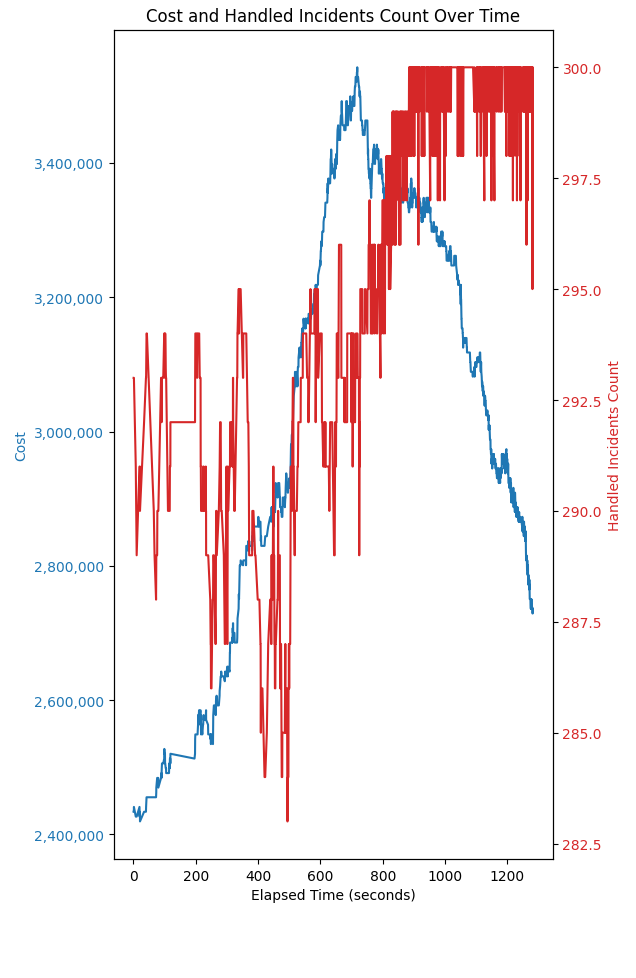
\includegraphics[width=0.7\textwidth,height=0.9\textwidth]{img/plots/sa_optimal.png}
  \centering
  \label{img:sa_optimal}
\end{figure}

Na grafu \ref{img:sa_optimal} vidíme průběh výpočtu.
Podobně jako v případě procházení z náhodného plánu jsou při vyšší teplotě navštěvovány horší plány v rámci explorace a od přibližně 
10 minuty (700 sekund) se postupně přechází do ladící fáze, která se chová podobně jako lokální prohledávání.
Program celkově běžel něco pod 30 minut i spolu s nalezením plánu optimálními tahy.
Nejlepší nalezený plán odbavuje 300 incidentů, stojí 2736133 a má naalokovaných 108 týmu a 133 vozidel.

\subsection{Porovnání metod}

V předchozích kapitolách jsme zformalizovali problém nalezení optimálního plánu záchranné služby a následně jsme navrhnuli několik metod řešící tuto úlohu.
Nalezené metody jsme aplikovali na model pražské záchranné služby a náhodně vygenerované sadě incidentů odpovídající, jak by se incidenty v Praze mohli reálně odehrávat.
V této kapitole shrneme klíčová pozorování z předešlého aplikování jednotlivých metod a následně mezi sebou metody porovnáme. 

Při analýze metody prohledávání plánů optimálními tahy jsme zjistili, že metoda je schopna poměrně rychle (7 minut) nalézt velmi kvalitní plán.
Lokální prohledávání z prázdného plánu je horší, a neumí z prázdného plánu nalézt podobně dobrý plán ani do hodiny.
Přednost lokálního prohledávání je totiž v schopnosti doladit nějaký už dost dobrý plán.
Kombinací lokálnílo prohledávání a prohledávání optimálními tahy jsme získali metodu,
která umí do 20 minut nalézt plán odbavující všechny incidenty a do téměř hodiny a půl dokonce lokálně optimální plán.

Tabu prohledávání není vhodnou metodou pro řešení našeho problému, protože je obtížné najít i jenom lokální optimum.
Nevyužije se tak lokální paměť, akorát se zbytečně kontroluje, zda neobsahuje sousední plán.
Simulované žíhání, narozdíl od tabu prohledávání, je vhodná metoda a podobně jako u lokálního prohledávání nejlépe funguje v kombinaci s metodou prohledávání optimálními tahy. 
Narozdíl od lokálního nebo tabu prohledávání, simulované žíhání neprozkoumává všechny sousední plány, a z toho důvodu konverguje o dost rychleji. 
Proto velmi dobře funguje i při prohledávání z náhodně vygenerovaného plánu.

Jakou konkrétně metodu použít velmi záleží na cíli, kterého chceme dosáhnout.
Pokud je žádoucí nalézt skutečně co nejlepší plán, odbavující nějakou danou sadu incidentů, tak je nejlepší zvolit kombinaci prohledávání optimálními tahy spolu s lokálním prohledáváním.
Ta nalezne velmi kvalitní plán, ale trvá poměrně dlouho.
Pokud je žádoucí nalézt dostatečně dobrý plán za kratší dobu, je lepší volbou spustit metodu prohledávání optimálními tahy spolu se simulovaným žíháním.
Simulované žíhání je rychlejší a bylo schopné nalézt kvalitní plán z plánu optimálního v ceně do 20 minut.
Přičemž při nižší finální teplotě by simulované žíhání konvergovalo k ještě lepšímu plánu, samozřejmě za cenu delšího běhu.

Nevýhodou prohledávání optimálními tahy je, že umí používat jenom účelovou funkci $q^{\text{Lex}}$.
Pokud bychom chtěli používat jinou účelovou funkci, například proto, že chceme nalézt plány, které odbavují jen o něco méně incidentů, ale jsou o dost levnější,
nemusí být prohledávání optimálními tahy vhodné použít.
V takovém případě je nejlepší z prázdného plánu nalézt dost dobrý plán simulovaným žíháním a následně nalézt jeho lokální optimum pomocí lokálního prohledávání.

\begin{table}[h!]
\centering
\begin{tabular}{|c|c|c|c|}
\hline
  \textbf{Metoda} & \textbf{Čas běhu} & \textbf{Cena} & \textbf{Odbavené incidenty} \\
\hline
  POT & 10:53 & 2469661 & 296 \\
\hline
  POT + LP & 32:52 & 2512864 & 300 \\
\hline
  POT + LP & 1:38:22 & 2188863 & 300 \\
\hline
  SŽ -- náhodný plán & 51:54 & 2124103 & 300 \\
\hline
  POT + SŽ & 21:15 & 2736133 & 300 \\
\hline
\end{tabular}
\caption{Shrnutí metod. POT značí prohledávání optimálními tahy, LP značí lokální prohledávání, SŽ značí simulované žíhání.}
\label{table:shrnutiMetod}
\end{table}

Pražská záchranná služba už je poměrně větší záchranná služba a spolu s použitím Google API a větší sady incidentů se jednalo o výpočetně dlouho trvající úlohu, avšak i tak
navrhnuté metody, pokud jsou správně použity, umí nalézt velmi kvalitní plány v průměru do hodiny (viz tabulka \ref{table:shrnutiMetod}).

